%!TEX root = batch-course.tex

%-------------------------------------------------
\section{Multiblock batch case study}
%-------------------------------------------------

\begin{frame}\frametitle{Case study: multiblock batch PLS model}

This case study will introduce a number of concepts, by example. We will see:
\begin{enumerate}

	\item	Multivariate characterization of product quality
	
	\item	Effect of initial conditions on product quality
		
	\item	Alignment of batch trajectories
	
	\item 	Troubleshoot problems: poor product quality
	
	\item 	Predictions of final quality attributes
	
	\item 	Overview of the monitoring concept
	
\end{enumerate} 
\end{frame}

\begin{frame}\frametitle{Case study: multiblock batch PLS model}
	
This case study is as complex as it gets: 

\begin{itemize}
	\item	Multiblock: 
	
		\begin{itemize}
			\item	\( \mathbf{Z} \): initial conditions
			
			\item	\( \mathbf{X} \): batch data
			
			\item	\( \mathbf{Y} \): CQAs
			
		\end{itemize}
		
	\item 	one of the blocks contains batch trajectories
	
	\item	we have a PLS model for the CQA predictions
\end{itemize}

\end{frame}

\begin{frame}\frametitle{Process background}

\begin{itemize}
	\item	Agricultural chemical production
	
	\item	Wet ``cake'' (solid with embedded solvent) charged to system and dried
	
	\item	Solvent is collected in an external, side tank
	
	\item	Chemical changes occur in the solid phase during drying 
	
	\item	3 phases in the recipe (more details later)

	\item	Operators can adjust some parameters
\end{itemize}

\end{frame}

\begin{frame}\frametitle{Process background}


	\begin{center}
		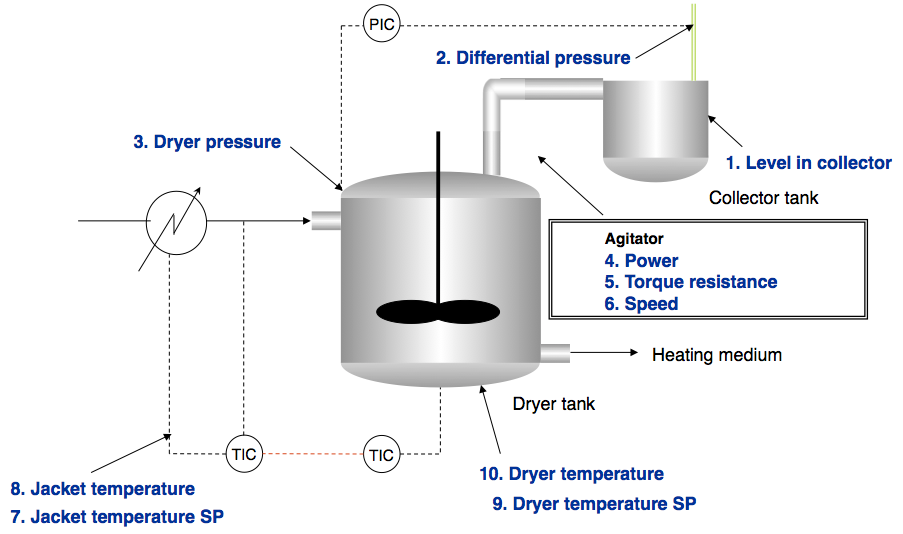
\includegraphics[width=\textwidth]{images/fmc/fmc-batch-system.png}
	\end{center}

\end{frame}

\begin{frame}\frametitle{More about the dataset}

\begin{itemize}
	\item	59 batches are present in the data set
	
	\begin{itemize}
		\item	initial conditions (plenty of missing values)
		
		\item	trajectories (unaligned)
		
		\item	CQAs (some missing values; lots of ``zeros'')
	\end{itemize}

	\item	We will go through the study in some detail and to learn about  {\color{myOrange}multiblock batch data analysis}
\end{itemize}

\end{frame}

\begin{frame}\frametitle{More about the dataset}

\begin{itemize}
	\item	13 batches are missing substantial initial chemistry information: excluded in all batches
	
	\item	46 batches remaining:
	
	\begin{itemize}
		\item	Good batches: labeled 1 to 33 (23 actual batch)

		\item	Abnormal batches: labeled 34 to 61 (17 actual batches)

		\item	High residual solvent batches: labeled 62 to 71 (6 actual batches)
	\end{itemize}
\end{itemize}

\end{frame}

\begin{frame}\frametitle{Characterizing product quality: CQAs, \( \mathbf{Y}\)}

\begin{itemize}
	\item	Product quality is a multivariate property
	
 	\item	It is expected to look at a PCA model of \( \mathbf{Y} \).  For example:
	
		\begin{itemize}
			\item	Mepron raw material properties (inputs)

			\item	Other models at GSK: you have likely done this before
			
			\item	Batch systems, and other CQAs are no different
		\end{itemize}
		
		\item	Look at these in the software
\end{itemize}

\end{frame}

\begin{frame}\frametitle{Characterizing product quality: CQAs, \( \mathbf{Y}\)}

\begin{itemize}
	\item	Raw data on 8 final product properties 
\end{itemize}

\begin{center}
	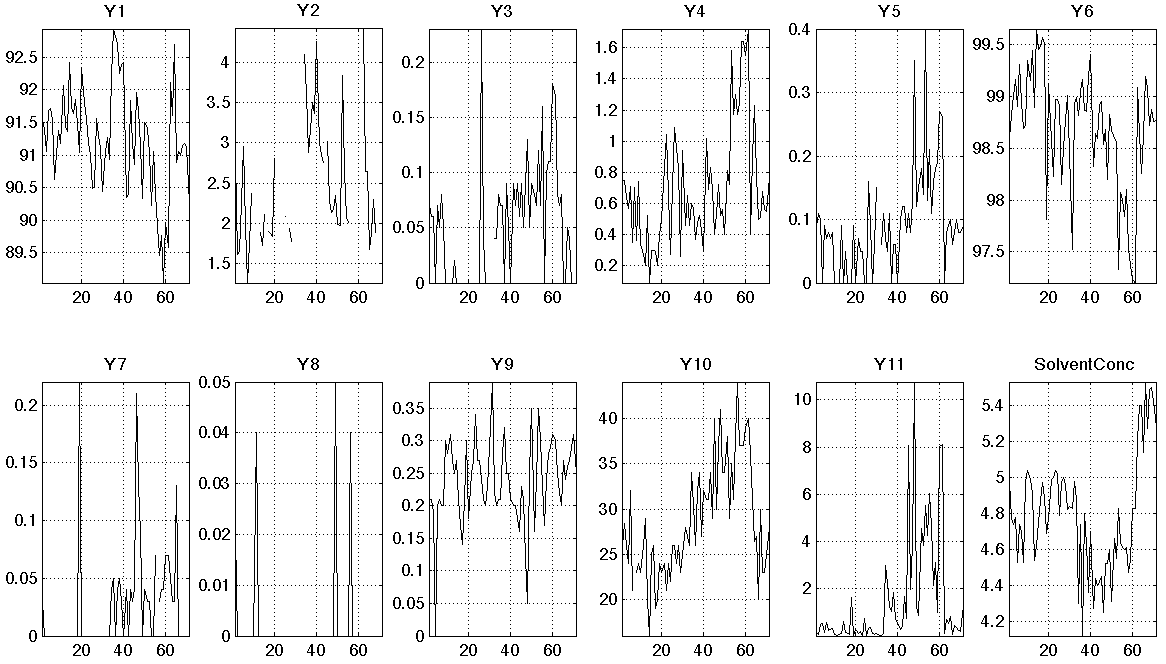
\includegraphics[width=\textwidth]{images/fmc/fmc-Z-raw-data.png}
\end{center}

\end{frame}

\begin{frame}\frametitle{Effect of initial conditions on product quality}

\begin{itemize}
	\item	Investigate the chemistry effect: \( \mathbf{Z}_\text{chem}\) effect on \( \mathbf{Y}\)
	
	\item	Weight of wet cake
\end{itemize}

\begin{center}
	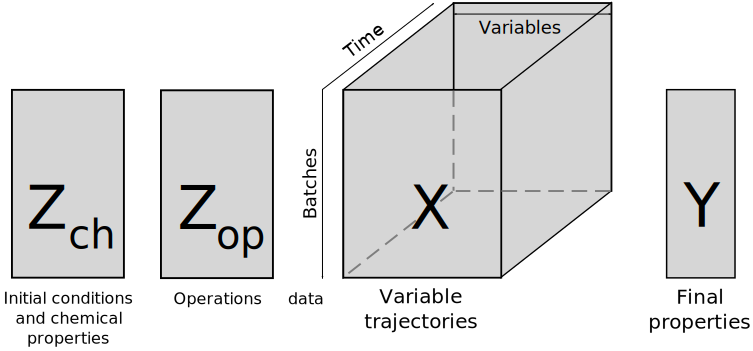
\includegraphics[width=\textwidth]{images/fmc/fmc-data-structure}
\end{center}

\end{frame}

\begin{frame}\frametitle{About the batch trajectories}

\begin{itemize}
	\item	10 trajectories measured online
	
	\item	3 phases:
	
	\begin{itemize}
		\item	solvent collection
		
		\item	temperature ramp
		
		\item	cooling down phase
	\end{itemize}
\end{itemize}
\begin{center}
	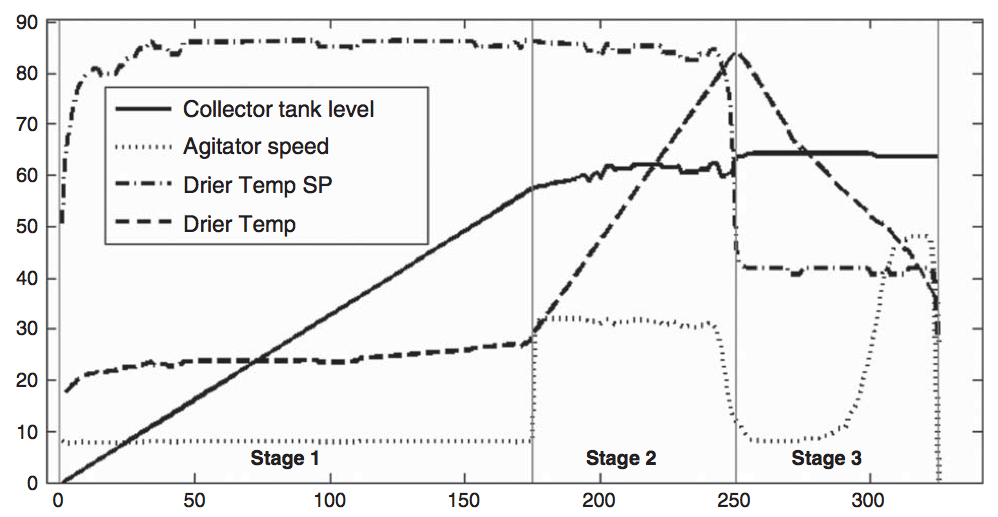
\includegraphics[width=\textwidth]{images/fmc/fmc-phases-4-trajectories.png}
\end{center}

\end{frame}

\begin{frame}\frametitle{Aligning the trajectories}

	\begin{itemize}
		\item	Done within each phase
	\end{itemize}
	\begin{center}
		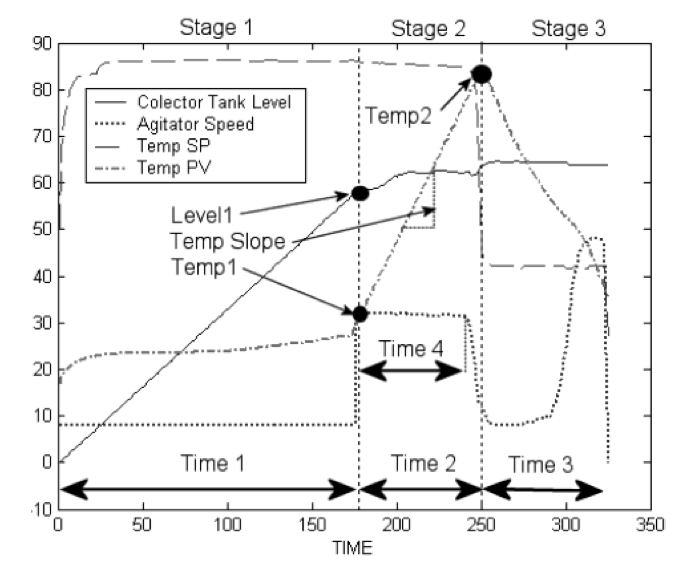
\includegraphics[width=0.7\textwidth]{images/fmc/fmc-alignment-points.png}
	\end{center}
	\begin{itemize}
		\item	Transfer alignment information to  \( \mathbf{Z}_\text{op}\)
	\end{itemize}
\end{frame}

\begin{frame}\frametitle{Aligning the trajectories}

	\begin{center}
		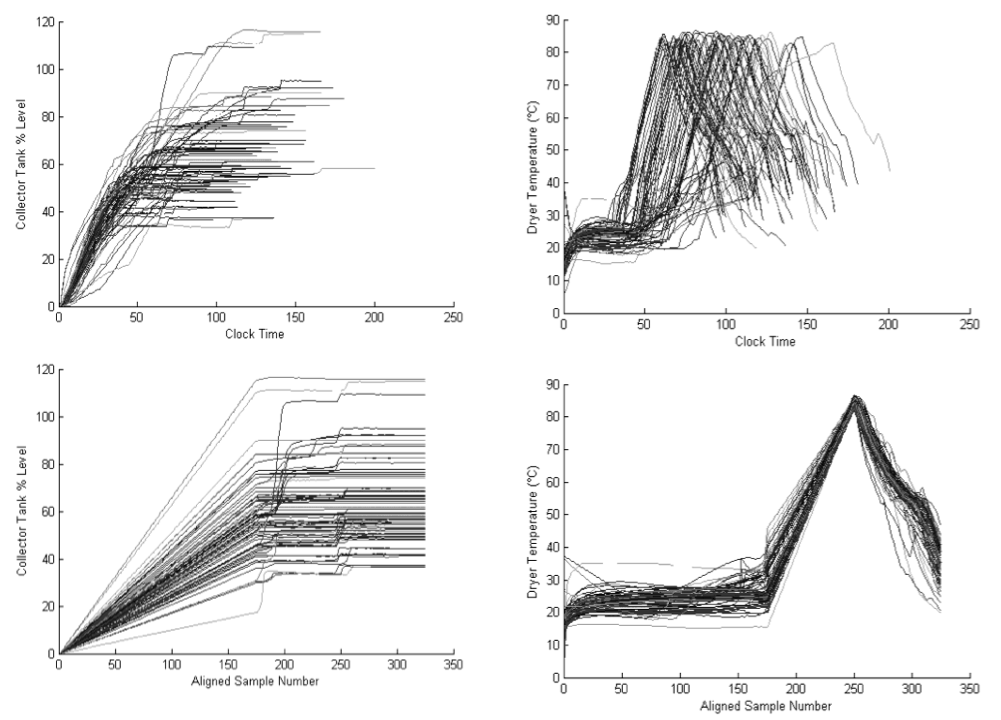
\includegraphics[width=\textwidth]{images/fmc/fmc-alignment-phase1-phase2.png}
	\end{center}

\end{frame}

\begin{frame}\frametitle{Aligning the trajectories}
	
	\begin{itemize}
		\item	Include time-distortion variable as a trajectory
	\end{itemize}
	\begin{center}
		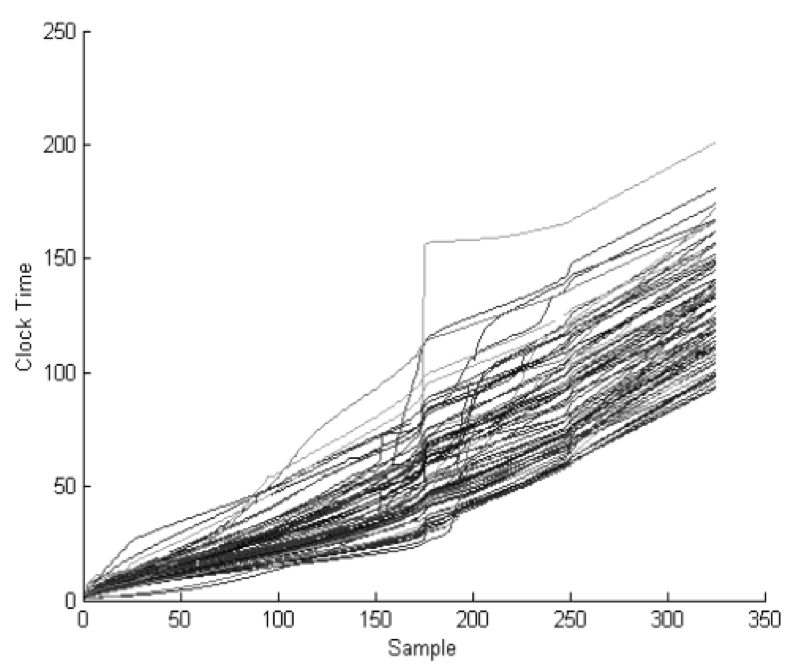
\includegraphics[width=0.75\textwidth]{images/fmc/fmc-distorted-time.png}
	\end{center}

\end{frame}

\begin{frame}\frametitle{A more complete analysis for product quality}

\begin{itemize}
	\item	Use data in \( \mathbf{Z}_\text{chem}\)
	
	\item 	Summary data in \( \mathbf{Z}_\text{op}\)
	
	\item 	Include actual trajectory information: \( \mathbf{X}\)
\end{itemize}

\begin{center}
	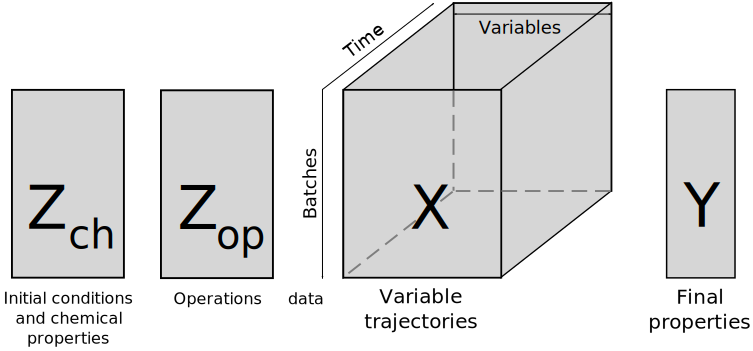
\includegraphics[width=\textwidth]{images/fmc/fmc-data-structure}
\end{center}

\begin{itemize}
	\item	Do this in the software.
\end{itemize}

\end{frame}

\begin{frame}\frametitle{Multiblock PLS}

\begin{itemize}
	\item	Use multiple \( \mathbf{X}\)-blocks
	
	\item	Always have a single \( \mathbf{Y}\) block
	
	\item	Calculated in the same way as ordinary PLS
	
	\item	Model interpretation is the same
\end{itemize}


\end{frame}

\begin{frame}\frametitle{What have we learned?}

\begin{itemize}
	\item	CQA's are always multivariate
	
	\item	Mastered troubleshooting of existing data using:
	
	\begin{itemize}
		\item	PCA
		
		\item	PLS
		
		\item	Batch PCA and PLS
		
		\item	Multi block datasets
	\end{itemize}
	
	\item	\textbf{Important skill}: more than 95\%  of latent variable models never go "on-line". Used for troubleshooting and learning.

	\item	\textbf{Another skill learned}: model interpretation 
\end{itemize}

\end{frame}